In this section, we discuss the performance and scalability of a
gravitational $N$-body simulation code implemented using FDPS. The
code is essentially the same as the sample code described in
section~\ref{sec:samplecode}, except for the following two differences
in the user code for the calculation of the interaction. First, here,
we used the expansion up to quadrupole moment, instead of
monopole-only one used in the sample code, to improve the
accuracy. Second, we used highly-optimized kernel developed using SIMD
builtin functions, instead of the simple one in the sample code.

We use the Plummer model \cite{1911MNRAS..71..460P} to realize
particle distribution at the initial time. We adopt $\theta=0.4$ for
the opening angle for the tree algorithm. In this paper, we present
the weak-scaling performance of the code with FDPS. Therefore we fixed
the number of particles per core to $250$ thousands.

\begin{figure}
  \begin{center}
%      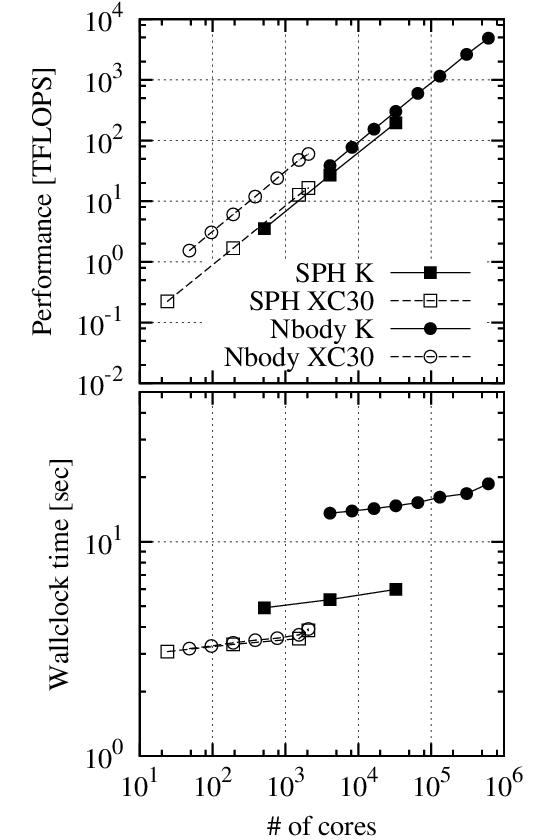
\includegraphics[width=8cm,bb=0 0 540 840]{../sandbox/tanikawa_box/figure/ws_sc15/bench.png}
      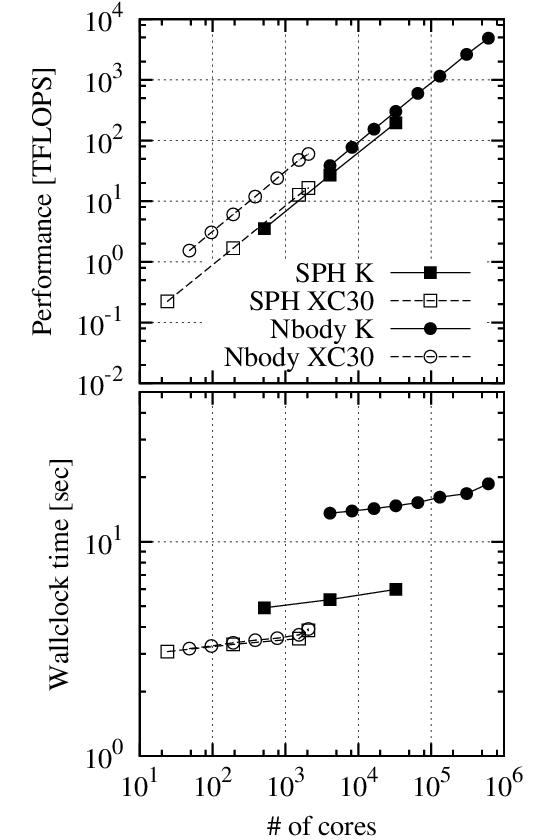
\includegraphics[width=7.5cm,bb=0 0 540 840]{../sandbox/tanikawa_box/figure/ws_sc15/bench.png}
  \end{center}
  \caption{Performance measured in the speed of the floating-point
    operation (top) and wallclock time per one timestep (bottom)
    plotted as functions of the number of cores. Filled and open
    points indicate the performance on K computer and Cray XC30,
    respectively. Square and circle points show the performance of our
    SPH simulation code and $N$-body simulation code, respectively.}
  \label{fig:benchdisk}
\end{figure}

We run our $N$-body simulation code on two platforms: K computer at
RIKEN Advanced Institute for Computational Science, and Cray XC30
(with Haswell processors) at National Astronomical Observatory of
Japan. The maximum numbers of cores we used are $612352$ cores
($76544$ nodes) on K computer, and $2064$ cores ($86$ nodes) on Cray
XC30. The run using $612352$ cores on K computer is almost a
full-system one, where the full-system run operates $663552$ cores.
Precision of floating point for interaction calculations is double on
K computer, and single on Cray XC30. The single floating point
precision is sufficient for the scientific calculation on this
field. Since the performance of the single floating point precision is
the same as that of the double one on K computer, we adopt the double
one for the calculation on K computer.

Filled and open circles in Figure~\ref{fig:benchdisk} show the
measured performance of our $N$-body simulation code. We can see the
measured efficiency and scalability are both very good on both
platforms. On K computer, efficiency is very close to 50\% for the
entire range of nodes. Wallclock time shows slight increase for larger
number of nodes, but this is due to the increase of the calculation
cost and not due to the degradation of the efficiency. The performance
on Cray XC30 is about $4$ times higher than that on K computer, since
the peak performance per core in single floating point precision on
Cary XC30 is about $5$ times higher than that in double floating point
precision on K computer

We compare the performance of our $N$-body simulation code with that
of GreeM code \cite{ishiyama:greem, ishiyama:gordonbell}. GreeM code
treats $N$-body simulation with TreePM algorithm, and was awarded the
2012 ACM Gordon Bell Prize. The wallclock times of GreeM and our codes
are $2.80 \times 10^{-11}$ and $1.16 \times 10^{-10}$
sec/step/particle. Our code using FDPS seems to be $4$ times slower
than GreeM. However, this is due to the difference of the algorithms
used. Since TreePM algorithm calculates forces from distant particles
by Fast Fourier Transform, the number of particle-particle
interactions in TreePM algorithm is much smaller than that in the tree
algorithm. Therefore, comparison of the wallclock time per interaction
is more fair. The wallclock time is $1.14 \times 10^{-14}$ (GreeM) and
$1.71 \times 10^{-14}$ (ours) sec/step/interaction. The performance is
comparable, even though the number of particles per node is smaller by
a factor of $6$. The performance of GreeM was measured for
$1.6$ million particles per core, while we used $250$ thousand
particles per core.

%%%% about comparison ...

%% ours     1.16 x 10^-10 sec/step/particle
%% ishiyama 2.80 x 10^-11 sec/step/particle

%% ours     1.71 x 10^-14 sec/step/interaction
%% ishiyama 1.14 x 10^-14 sec/step/interaction

%B\'edorf \textit{et al.}\cite{Bedorf:2014:PGT:2683593.2683600}
%reported the wallclock time of 4 seconds for their 27-billion
%particle simulation on the Titan system with 2048 NVIDIA Tesla K20X,
%with the theoretical peak performance of 8PF (single precision, since
%single precision us used for interaction calculation). This
%corresponds to 0.8 billion particles per second per petaflops. Our
%code on K computer requires 15 seconds on 16384 nodes (2PF
%theoretical peak), resulting in 1 billion particles per second per
%petaflops. Therefore, we can conclude that our FDPS code achieved the
%performance slightly better than one of the best codes specialized to
%gravitational $N$-body problem.

% LocalWords:  FDPS superparticle monopole quadrupole SIMD builtin Hernquist IC
% LocalWords:  Frenk NFW EP scalability TPP PFLOPS NVIDIA kpc axisymmetric pc
% LocalWords:  GalacticICS Gyrs timestep edorf et al petaflops Wallclock
% LocalWords:  wallclock
